\documentclass[twocolumn]{article}
\usepackage{styles/example,amsmath,booktabs,graphicx}
\title{A reproducible manuscript workflow\\\large Synthetic project for software verification}
\author{awesome-latex-skills maintained examples}
\date{}
\begin{document}
\maketitle
\begin{abstract}
This multi-file manuscript is a synthetic software example, not a scientific
result or an official venue template. It contains grouped table headers,
multi-panel illustrations, a bibliography, an appendix and a Chinese companion.
All displayed observations are supplied toy values. Source repair must retain
their precision, mathematical definitions and uncertainty.
\end{abstract}
\section{Introduction}\label{sec:introduction}
Reproducible manuscript tooling should retain source evidence through repairs.
This example uses documented equation environments~\cite{amsguide}.
Figure~\ref{fig:panels} illustrates the supplied workflow, and
Table~\ref{tab:results} lists illustrative observations.
The diagram does not constitute an architectural claim about a real model.

\section{Definitions}\label{sec:methods}
The toy objective is
\begin{equation}
\mathcal{L}=\mathcal{L}_1+\lambda\mathcal{L}_2,\qquad\lambda=0.5.
\label{eq:objective}
\end{equation}
The encoder maps inputs to an embedding space; a separate generative model
samples a latent space. These terms are retained as distinct definitions.
No causal or universal performance claim is supplied.
\begin{figure}[htbp]
\centering
\begin{minipage}{0.8\linewidth}
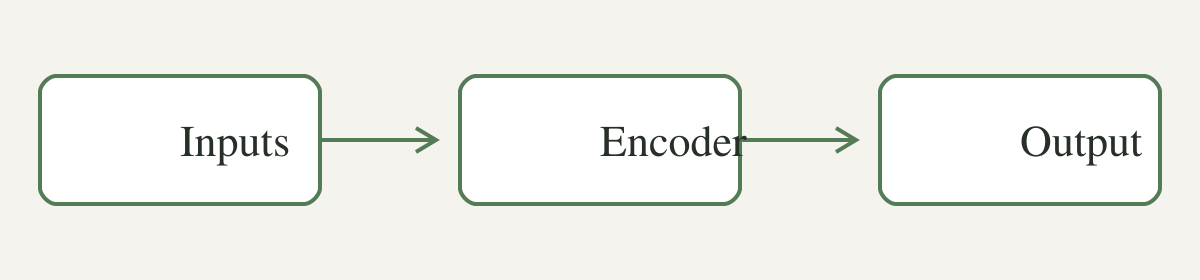
\includegraphics[width=\linewidth]{figures/panel}\\
\small (a) Supplied schematic
\end{minipage}\par\medskip
\begin{minipage}{0.8\linewidth}
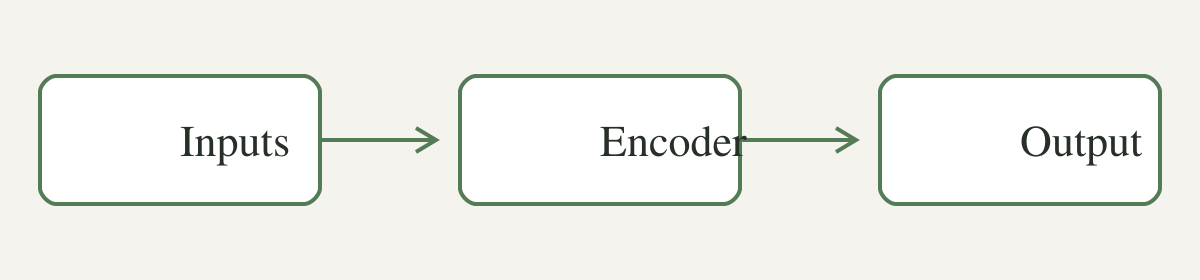
\includegraphics[width=\linewidth]{figures/panel}\\
\small (b) The same illustrative pipeline
\end{minipage}
\caption{Two synthetic panels; neither implies measured model behavior.}
\label{fig:panels}
\end{figure}

\section{Illustrative observations}\label{sec:results}
Under the supplied toy setting on \datasetname{}, the values are shown in
Table~\ref{tab:results}. \textbf{These are not research findings.}
\begin{table}[htbp]
\centering\small
\caption{Supplied synthetic values with retained precision.}\label{tab:results}
\begin{tabular}{@{}lrrl@{}}
\toprule
Method & \multicolumn{2}{c}{Score (\%)} & Status\\
\cmidrule(lr){2-3}
& Mean & Spread &\\
\midrule
Alpha & 76.10 & 0.30 & toy\\
Beta & 78.20 & 0.40 & toy\\
Variant & -{}- & & n/a\\
\bottomrule
\end{tabular}
\end{table}
The Variant Spread cell is blank; it is not zero.
No uncertainty distribution, repetitions or significance test was supplied.

\section{Scope and limitations}\label{sec:discussion}
The illustrative observations apply only to the supplied toy setting.
They do not establish generalization or a causal mechanism.
\par\noindent[UNCERTAIN: timing protocol has not been supplied.]
The software workflow can verify compilation and literal evidence; authors
must review scientific meaning and the requirements of their actual venue.

\bibliographystyle{plain}
\bibliography{references}
\appendix
\section{Reproduction record}\label{sec:appendix}
Keep the original project, selected engine and bibliography backend, source
fingerprints, logs and PDFs. Equation~\eqref{eq:objective} retains its supplied
weight. The bibliography entry cites official documentation, not evidence
for the toy observations. No hidden experimental protocol is inferred.

\end{document}
